%!TEX root = Thesis_main.tex
\begin{appendices}
%%%%%%%%%%%%%%%%%%% AAAAA %%%%%%%%%%%%%%%%%%%%%
\chapter{Super Mega Bot Datasheet}
\label{appA}


\begin{figure}[h]
	\begin{center} 
		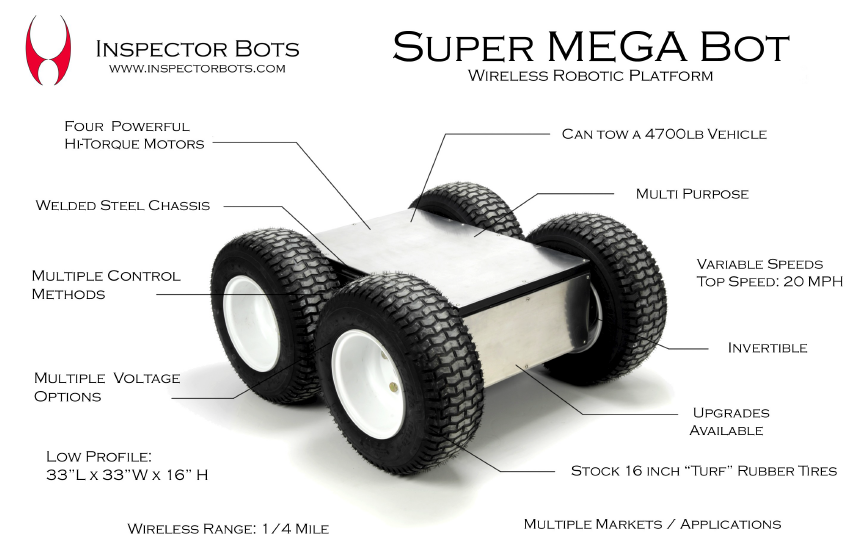
\includegraphics[scale=0.6]{SuperMegaBot}
		\centering
		\label{fig:SuperMegaBot} 
	\end{center}
\end{figure}


Its base model comes with:\\
•	Chassis: Powder Coated Steel and Aluminum \\
•	Dimensions: 84cm L x 84cm W x 40.64cm H, Weight: 109 kg\\
•	Drive: Four Electric Motors\\
•	Load Capacity: 113,5 kg\\
•	Speed Controllers: RoboteQ 2x VDC2450\\
•	Speed: 0-16 km/h \\
•	Suspension: Rigid\\
•	Tires: Interchangeable, Pneumatic, 40.64cm Diameter Turf Tires\\
\url{https://www.youtube.com/watch?v=3X8IWnR1QDI}


%%%%%%%%%%%%%%%%%%% BBBBB %%%%%%%%%%%%%%%%%%%%%
\chapter{UR5 Datasheed}
\label{appB}
In the following table the specifications given by Universal Robots are stated. 
\begin{table}
	\begin{tabular}{p{4cm} | p{3cm} p{3cm}}
		\hline
		Performance & \multicolumn{2}{l}{ } \\
		\hline \hline
		Repeatibility & \multicolumn{2}{l}{$\pm$ 0.1 mm} \\
		Ambient temperature range & \multicolumn{2}{l}{0-50°} \\
		Power Consumption  & \multicolumn{2}{l}{Min 90W, Typical 150W, Max 325W} \\
		Collaboration operation & \multicolumn{2}{l}{15 advanced adjustable safety functions} \\
		\hline \hline
		Specifications & \multicolumn{2}{l}{ }\\
		\hline \hline 
		Payload & \multicolumn{2}{l}{5 kg} \\
		Reach & \multicolumn{2}{l}{850 mm} \\
		Degrees of freedom & \multicolumn{2}{l}{6 rotating joints} \\
		Programming & \multicolumn{2}{l}{Polyscope graphical user interface on 12 inch touchscreen} \\
		\hline \hline
		Movement & & \\
		\hline 
		& Working range & Maximum speed \\
		\hline \hline
		Base & $\pm$ 360°  & $\pm$ 180°/sec \\
		Shoulder & $\pm$ 360° & $\pm$ 180°/sec \\
		Wrist1 & $\pm$ 360° & $\pm$ 180°/sec \\
		Wrist2 & $\pm$ 360° & $\pm$ 180°/sec \\
		Wrist3 & $\pm$ 360° & $\pm$ 180°/sec \\
		Typical tool & & 1m/sec \\
		\hline \hline
		Physical & \multicolumn{2}{l}{ }\\
		\hline \hline
		Footprint & \multicolumn{2}{l}{\o 149mm} \\
		Materials & \multicolumn{2}{l}{Aluminium, PP Plastics} \\
		Weight (with cable) & 18.4 kg 
	\end{tabular}
\end{table}


%%%%%%%%%%%%%%%%%%% CCCCC %%%%%%%%%%%%%%%%%%%%%
\chapter{Interior Point OPTimizer (IPOPT)}
\label{appC}

\end{appendices}





